\section{Verification, Validation, and Simulation Results}
\label{sec:results}

This chapter separates verification of implemented equations, comparison with public flight evidence, and navigation error against simulation truth. The final nominal record R1 uses seed 1, $0.01\,\mathrm{s}$ maximum step, 100 Hz IMU and $0.1\,\mathrm{s}$ output; its original path is given in Appendix~\ref{sec:appendix-reproduction}. All 31 runtime/data fingerprints match the reviewed source. The shared archive and \path{report/reproduce.py} regenerate the result panels and numerical macros without another full-flight integration. The provenance ledger \path{report/figure_sources.json} records source hashes and extracted metrics.

\subsection{Model verification and state continuity}
The vehicle/navigation suite contains 130 passing assertion-based tests; the environment suite adds 41. They cover mass aggregation and derivatives, force-arm signs, fixed-mass free fall and constant-moment rotation, rotating Body storage, propellant bounds, aerodynamic flow reversal/damping, event guards, separation and two-child execution. Navigation tests add tolerance-based finite differences for the 30-state transition, SO(3) right Jacobian and sensor sensitivities, as well as startup epoch, delayed-attitude, gate and colored-noise checks. The legacy print-only diagnostics are not counted as assertion tests. These checks establish behavior in their fixtures, rather than agreement with real hardware.

At $144\,\mathrm{s}$, parent mass is $211019.374\,\mathrm{kg}$ and child masses are $91089.374$ and $119930.000\,\mathrm{kg}$. Their mass residual is zero. Relative linear- and angular-momentum residuals are $9.95\times10^{-19}$ and $9.54\times10^{-12}$; recombined-CG position error is $4.66\times10^{-10}\,\mathrm{m}$. These satisfy the numerical criteria of Section~\ref{sec:vehicle} for the assumed zero-impulse map. Both child states remain finite and are propagated without replacing their inherited initial conditions. Conservation under an assumed map does not establish the accuracy of real separation impulses or discarded hardware.

\subsection{Continuous mission and separated trajectories}
Figure~\ref{fig:results-flight} shows the complete generated sequence, and Figure~\ref{fig:results-trajectories} distinguishes the two children. Shutdown completes at 141 and separation occurs at $144\,\mathrm{s}$. The three return burns and their measured consumption appear in Table~\ref{tab:burn-results}; their endpoints are integration results of the conditions in Section~\ref{sec:mission-exec}.

\par\medskip\noindent\begin{minipage}{\linewidth}
\centering
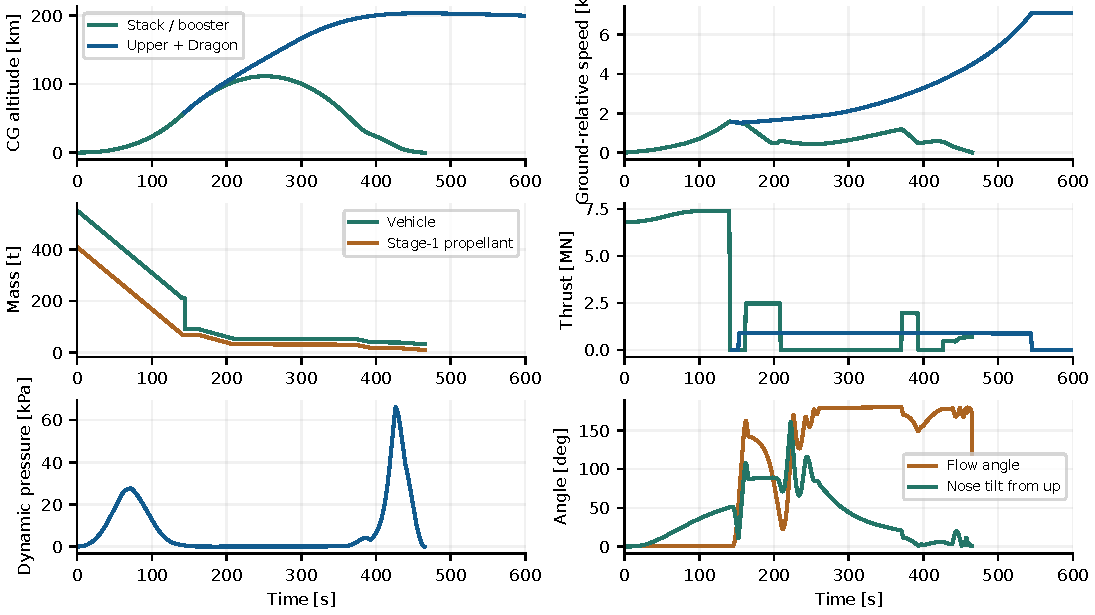
\includegraphics[width=\linewidth]{images/results_flight_profiles.pdf}
\captionof{figure}{R1 continuous flight. Green denotes stack/booster and blue the upper child where both are shown. The mass jump is a change of tracked configuration at separation. Flow angle near $180^\circ$ means engine-first relative flow, not attitude-estimation error. The trajectories use project commands and truth-state feedback.}
\label{fig:results-flight}
\end{minipage}\par\medskip

\par\medskip\noindent\begin{minipage}{\linewidth}
\centering\small
\begin{tabular}{@{}lrrl@{}}
\toprule
Burn & Start--end [s] & Consumed [t] & End condition \\
\midrule
Boostback & 161.00--208.81 & 37.982 & Fuel/duration planning cap \\
Entry & 370.14--392.95 & 14.158 & Speed target, then smooth shutdown \\
Landing & 426.16--465.083 & 7.818 & First contact \\
\bottomrule
\end{tabular}
\captionof{table}{Observed R1 return-burn intervals and fuel consumption. Boostback reaches its planning cap rather than the 500 m predicted-miss target. Its recorded predicted miss at burn end is about 3.97 km; later phases provide additional correction.}
\label{tab:burn-results}
\end{minipage}\par\medskip

The ascent dynamic-pressure maximum is $27.62\,\mathrm{kPa}$ at $71.9\,\mathrm{s}$, compared with the approximate $75\,\mathrm{s}$ preflight marker. The full-flight maximum is instead $66.16\,\mathrm{kPa}$ near landing ignition at $426.3\,\mathrm{s}$; the two maxima must not be confused. Between entry shutdown and landing ignition, gravity accelerates the unpowered descending booster again, explaining the late rise in its speed. Landing then brakes it to the contact state.

\par\medskip\noindent\begin{minipage}{\linewidth}
\centering
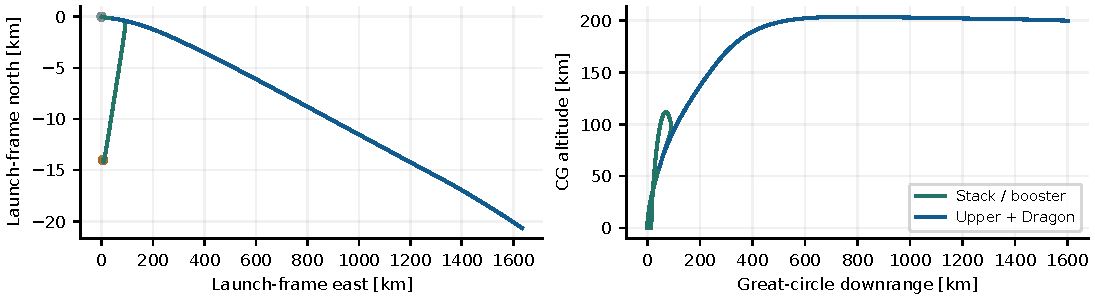
\includegraphics[width=\linewidth]{images/results_trajectories.pdf}
\captionof{figure}{R1 separated paths: launch-frame horizontal projection and altitude against spherical downrange. The marked horizontal points are launch and the assumed return target. The booster returns while the upper-stage/Dragon child continues downrange from the same separation event.}
\label{fig:results-trajectories}
\end{minipage}\par\medskip

Figure~\ref{fig:results-kinematics} completes the kinematic outputs requested in the assignment \cite[slide 5]{project2}. Great-circle downrange is $R_E\arccos(\hat{\vect r}\cdot\hat{\vect r}_{\mathrm{pad}})$; it is distance from the pad, not accumulated path length. Flight-path angle is $\gamma=\operatorname{atan2}(v_r,\lVert\vect v-v_r\hat{\vect r}\rVert)$, where $v_r=\vect v\cdot\hat{\vect r}$ and $\vect v$ is CG Earth-relative velocity. Actual rate magnitude peaks at $17.825^\circ\,\mathrm{s^{-1}}$ at $223.7\,\mathrm{s}$ in return coast. This is compatible with the per-axis desired-rate clip of Section~\ref{sec:mission-exec}; it is not a state-norm limit.

\par\medskip\noindent\begin{minipage}{\linewidth}
\centering
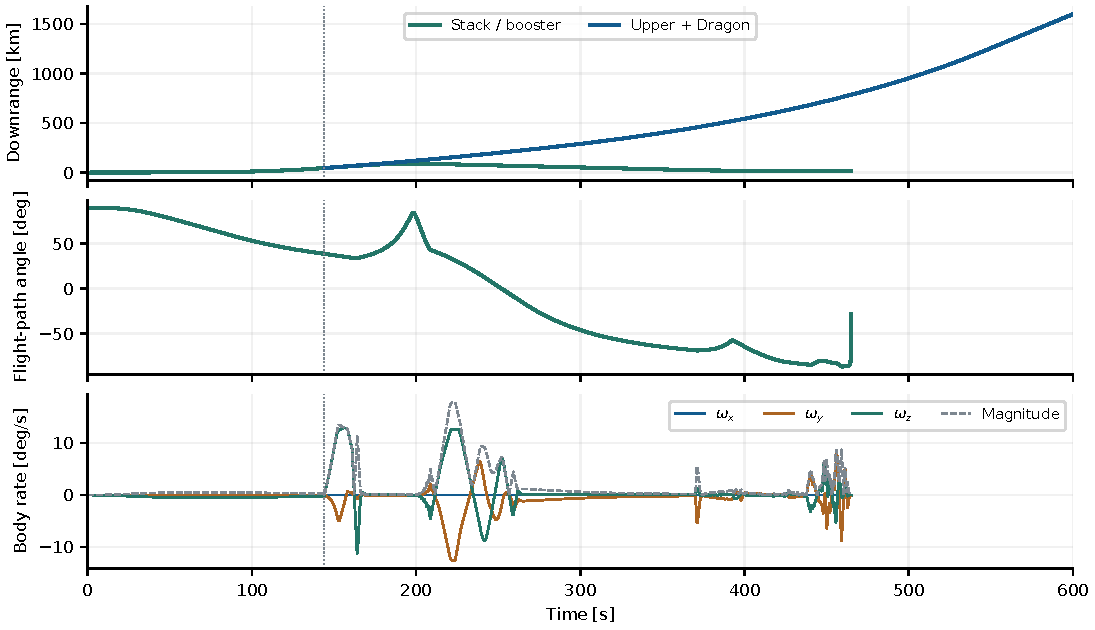
\includegraphics[width=\linewidth]{images/results_kinematics.pdf}
\captionof{figure}{R1 downrange for both children, stack/booster flight-path angle, and true Body-rate components/magnitude. Positive flight-path angle denotes outward motion; negative denotes descent. The angle is omitted below $1\,\mathrm{m\,s^{-1}}$, where direction is poorly defined. The dotted line marks separation. The post-boostback coast turn explains the largest rate excursion.}
\label{fig:results-kinematics}
\end{minipage}\par\medskip

Table~\ref{tab:landing-results} evaluates the project limits at contact. Contact occurs at $465.0827\,\mathrm{s}$ with $8.931\,\mathrm{t}$ of stage-1 propellant remaining. The ground condition applies to the lowest leg tip, so the CG remains above zero altitude. The upper child continues to $600\,\mathrm{s}$, reaching $199.694\,\mathrm{km}$ and $7.097\,\mathrm{km\,s^{-1}}$, with $5.472\,\mathrm{t}$ of propellant. This is a successful project scenario, not proof of SpaceX guidance reconstruction or validated orbital insertion.

\par\medskip\noindent\begin{minipage}{\linewidth}
\centering\small
\begin{tabular}{@{}lrr@{}}
\toprule
Acceptance metric & R1 result & Project limit \\
\midrule
Vertical speed [$\mathrm{m\,s^{-1}}$] & 0.4975 & 2 \\
Horizontal speed [$\mathrm{m\,s^{-1}}$] & 0.9016 & 1 \\
Tilt [deg] & 0.5349 & 5 \\
Angular-rate magnitude [$\mathrm{deg\,s^{-1}}$] & 0.01289 & 1 \\
Horizontal target error [m] & 3.306 & 10 \\
\bottomrule
\end{tabular}
\captionof{table}{R1 mission-level contact metrics. Speeds and target error use the structural-base state; ground contact is tested at the lowest leg tip. Ground contact and deployed legs are also required and satisfied. These are assumed project limits; horizontal speed has the smallest fractional margin.}
\label{tab:landing-results}
\end{minipage}\par\medskip

\subsection{Comparison with the ascent reference}
\label{sec:ascent-results}
Figure~\ref{fig:results-reference} compares 140 retained video-derived samples over $0$--$139.973\,\mathrm{s}$ \cite{crs10webcast,crs10telemetry}. Altitude RMSE is $1.577\,\mathrm{km}$ and speed RMSE $18.46\,\mathrm{m\,s^{-1}}$. At the last sample, simulated altitude is $54.628\,\mathrm{km}$ versus $59.400\,\mathrm{km}$, a $-8.03\%$ difference; speed is $1574.19$ versus $1609.44\,\mathrm{m\,s^{-1}}$, a $-2.19\%$ difference.

\par\medskip\noindent\begin{minipage}{\linewidth}
\centering
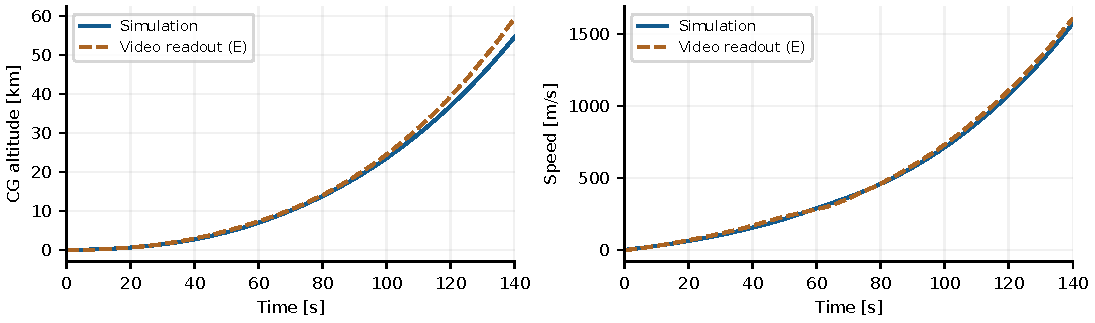
\includegraphics[width=\linewidth]{images/results_ascent_reference.pdf}
\captionof{figure}{R1 ascent against the E-class digitized broadcast readouts. This is the same record used to calibrate the ascent operating point/pitch timescale. Model CG altitude and ground-relative speed are compared with readouts whose detailed datum/frame conventions are not independently established.}
\label{fig:results-reference}
\end{minipage}\par\medskip

The comparison supports quantitative calibration within the retained ascent interval. It does not independently validate the tuned parameters, establish internal mass properties, or validate the return/upper-stage commands. Readout rounding, digitization and speed-frame uncertainty also limit interpretation of the residuals as pure physical-model error. The fairing-to-Dragon aerodynamic transfer and mixed-source vehicle data remain model uncertainties.

\subsection{Navigation accuracy and statistical diagnostics}
\label{sec:nav-results}
The gyro-driven navigation result is evaluated at the fixed IMU station, not at the moving CG. Equation~\eqref{eq:error-metrics} defines the three-dimensional position RMS and shortest quaternion-error angle used below:
\begin{equation}
 \mathrm{RMS}_p=\sqrt{\frac1N\sum_{k=1}^{N}\lVert\hat{\vect p}_k-\vect p_{\mathrm{true},k}\rVert^2},\qquad
 e_q=2\arccos\!\left(\left|\hat{\vect q}^{\mathsf T}\vect q_{\mathrm{true}}\right|\right).
\label{eq:error-metrics}
\end{equation}
The quaternion inner product is clamped numerically to $[0,1]$. Velocity RMS uses the corresponding velocity error. Figure~\ref{fig:results-navigation} shows accuracy and uncertainty diagnostics together.

\par\medskip\noindent\begin{minipage}{\linewidth}
\centering
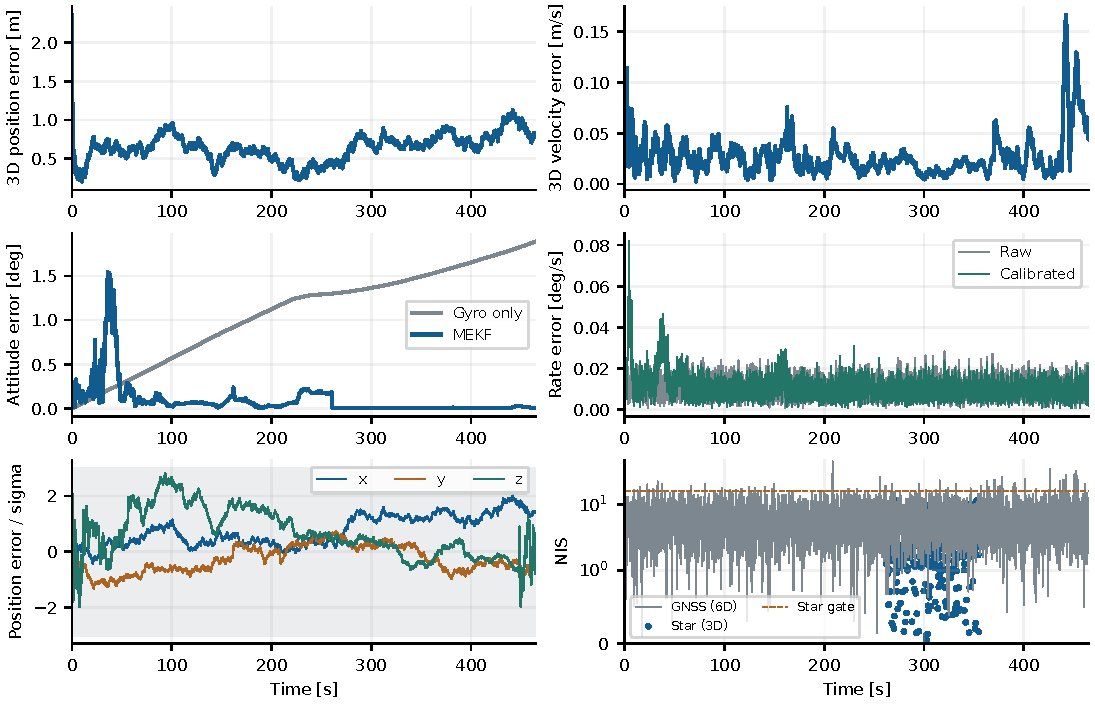
\includegraphics[width=\linewidth]{images/results_navigation.pdf}
\captionof{figure}{R1 navigation at the IMU station: position/velocity errors, estimated versus unaided attitude error, raw/calibrated angular-rate errors, normalized position errors and innovation diagnostics. The shaded interval is $\pm3$ reported standard deviations. The star gate is unchanged at 16.27; GNSS NIS is diagnostic. Accuracy, covariance consistency and rate calibration are assessed separately.}
\label{fig:results-navigation}
\end{minipage}\par\medskip

Position RMS is $\PositionRMS\,\mathrm{m}$, velocity RMS $\VelocityRMS\,\mathrm{m\,s^{-1}}$, and attitude RMS $\AttitudeRMS^\circ$. Attitude error peaks at $\AttitudePeak^\circ$ near $\AttitudePeakTime\,\mathrm{s}$ and ends at $\AttitudeFinal^\circ$, versus $\GyroOnlyFinal^\circ$ for the paired unaided gyro quaternion. These are simulation-truth errors under the declared alignment and sensor settings.

The archived earlier filter supplies a controlled comparison: both truth trajectories are byte-identical to R1 and all common raw sensor fields are identical sample by sample. Its position/velocity/attitude RMS values are $0.881\,\mathrm{m}$, $0.1354\,\mathrm{m\,s^{-1}}$ and $0.456^\circ$. The improvement measures the combined estimator changes of Section~\ref{sec:navigation}; it does not isolate each change's contribution. Physical flight and guidance are unchanged.

LiDAR supplies 496 valid corrections. All $\StarAccepted$ valid star exposures are accepted, with $\StarRejected$ rejected; the gate remains 16.27. Their mean and maximum NIS are $\StarNIS$ and $\StarMaxNIS$, and mean six-component GNSS NIS is $\GnssNIS$. Position errors remain inside reported $\pm3\sigma$ at every recorded epoch on all three axes. These correlated time samples are diagnostics, not independent coverage probabilities. All 4652 stored $30\times30$ covariance matrices are finite and symmetric, with minimum eigenvalue $1.01\times10^{-12}$; full matrices are archived for inspection.

Across $\RateSamples$ synchronized IMU/output epochs, calibrated angular-rate RMS is $\CalibratedRateRMS^\circ\,\mathrm{s^{-1}}$, compared with raw $\RawRateRMS^\circ\,\mathrm{s^{-1}}$. The nominal true gyro scale/cross-axis errors are zero; estimating them adds finite-sample uncertainty and does not guarantee improved instantaneous rates. The output remains an estimate of angular velocity, but this nominal case alone is insufficient evidence of calibration benefit. The independent nonzero-error test below supplies that evidence within its own excitation conditions.

\subsection{Independent navigation and covariance tests}
The executable \path{report/validate_navigation.py} supplies controlled truths independently of the CRS-10 trajectory. It runs a three-axis accelerometer-scale fixture, an analytic three-axis attitude fixture with nonzero gyro calibration errors, and 20 independent position/covariance realizations. Tolerances and fixture settings are explicit in Table~\ref{tab:independent-navigation} and Appendix~\ref{sec:appendix-reproduction}; all ten stored checks, including the isolated RK4 test below, pass. Figure~\ref{fig:independent-navigation} shows convergence and the independent final-epoch errors.

\par\medskip\noindent\begin{minipage}{\linewidth}
\centering\small
\begin{tabularx}{\linewidth}{@{}p{.34\linewidth}XX@{}}
\toprule
Independent check & Measured result & Acceptance criterion \\
\midrule
Accelerometer scale / bias error norm & $3.02\times10^{-5}$ / $3.79\times10^{-5}\,\mathrm{m\,s^{-2}}$ & $<4\times10^{-4}$ / $<0.002\,\mathrm{m\,s^{-2}}$ \\
Final attitude / gyro bias error norm & $0.00363^\circ$ / $1.21\times10^{-6}\,\mathrm{rad\,s^{-1}}$ & $<0.03^\circ$ / $<2\times10^{-5}\,\mathrm{rad\,s^{-1}}$ \\
Gyro scale / cross-axis error norm & $1.88\times10^{-4}$ / $8.06\times10^{-5}\,\mathrm{rad}$ & $<4\times10^{-4}$ / $<8\times10^{-4}\,\mathrm{rad}$ \\
Late-window raw / calibrated rate RMS & $0.03751/0.01004^\circ\,\mathrm{s^{-1}}$ & Calibrated RMS smaller \\
Position ANEES, 20 independent trials & $2.377$ (3 coordinates) & 95\% interval $[2.024,4.165]$ \\
GNSS mean NIS in the same fixture & $5.957$ (6 components) & Engineering check $5.5$--$6.5$ \\
\bottomrule
\end{tabularx}
\captionof{table}{Independent navigation checks. Error norms compare estimated parameters with injected truth. Numerical calibration tolerances and the NIS band are chosen engineering criteria; the ANEES interval has a stated chi-square statistical interpretation.}
\label{tab:independent-navigation}
\end{minipage}\par\medskip

For $M=20$ independent final position errors, $\mathrm{ANEES}=M^{-1}\sum_i\vect e_i^{\mathsf T}\mat P_{p,i}^{-1}\vect e_i$. The nominal 95\% acceptance interval is $[\chi^2_{60,0.025},\chi^2_{60,0.975}]/20$ \cite{nistchisquare}. A single final epoch per independently sampled prior/noise realization avoids treating one correlated time series as an ensemble. The result is compatible with this position-marginal test, not proof of whole-flight 30-state consistency. The gyro fixture accepts 1799 and rejects 2 of 1801 valid star exposures at the same gate; no requirement for zero stochastic rejections is imposed.

\par\medskip\noindent\begin{minipage}{\linewidth}
\centering
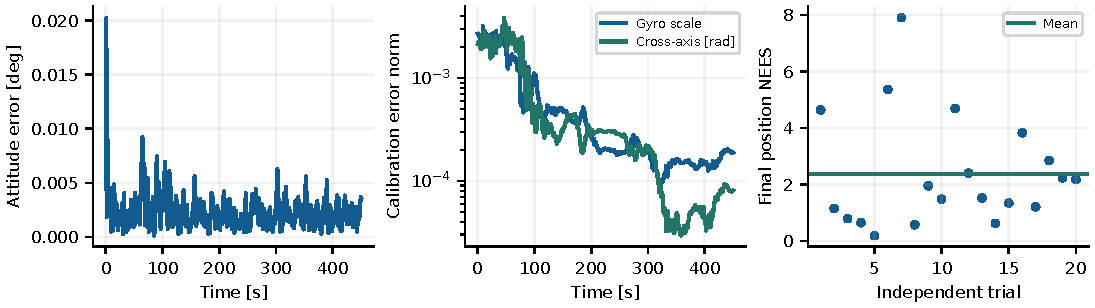
\includegraphics[width=\linewidth]{images/results_navigation_validation.pdf}
\captionof{figure}{Independent navigation fixtures. Left and middle: bounded analytic three-axis attitude with nonzero gyro bias, scale and cross-axis errors; calibration errors converge under the specified excitation and aiding. Right: one final position NEES per independent realization, with their mean. This is separate from the nominal mission and is not a wind/landing robustness ensemble.}
\label{fig:independent-navigation}
\end{minipage}\par\medskip

\subsection{Numerical sensitivity and demonstrated scope}
A saved variant, \path{results/two-stage-final-check}, uses $0.05\,\mathrm{s}$ steps and 20 Hz IMU with matching compared core-physics input hashes. It also lands, at $465.1900\,\mathrm{s}$, with target error $6.171\,\mathrm{m}$ and tilt $1.806^\circ$, versus R1's $3.306\,\mathrm{m}$ and $0.535^\circ$. The plan differs in IMU rate and the integration step is also changed. This is a joint step/clock diagnostic, not an isolated RK4 convergence-order study; contact metrics remain numerically sensitive even when both cases pass.

An isolated constant-spin rigid-body fixture tests RK4 without sensor, guidance or event clocks. Against the exact quaternion at $10\,\mathrm{s}$, steps $0.4$, $0.2$ and $0.1\,\mathrm{s}$ give attitude errors $5.1093\times10^{-7}$, $3.1983\times10^{-8}$ and $1.9997\times10^{-9}\,\mathrm{rad}$. Step-halving orders are 3.9977 and 3.9994, within the selected $[3.8,4.2]$ criterion. This verifies fourth-order behavior in the smooth rotation fixture; it does not establish mission-wide convergence through discrete events.

A separate static allocation check quantifies the dry-CG uncertainty of Section~\ref{sec:vehicle}. With an assumed $10\,\mathrm{t}$ of propellant remaining, the booster mass is $32.2\,\mathrm{t}$ and nominal CG station $16.211\,\mathrm{m}$. Moving the unallocated $6450\,\mathrm{kg}$ centroid over the declared $4.0$--$40.8\,\mathrm{m}$ interval shifts the combined CG by up to $\pm3.686\,\mathrm{m}$. For an explicitly assumed $1\,\mathrm{kN}$ transverse force at a fixed structural station, this changes its CG moment by up to $\pm3.686\,\mathrm{kN\,m}$. These are conditional allocation effects, not flight-error confidence bounds.
